\chapter{Introduction to Diffeomorphic Image Registration}\label{ch:introduction}


\begin{flushright}
	%\emph{Accurate and exact computations: the entrance into knowledge \\ of all existing things \\ and all obscure secrets.\\
	%	- Ahmes, 1800 B.C.}
		\emph{The series is divergent, therefore we may be able \\ to do something with it.}\\
			- Oliver Heaviside
\end{flushright}



\section{Toward an ill-posed Problem}

%Two instruments from Machine Vision and Image Processing are mostly utilized in Medical Imaging to reveal internal features and compare anatomies: segmentation and registration. Segmentation consists in enhance contours, detect edges and reveal hidden structure while registration is the .\\

The process of determining correspondences between two or more images acquired from patients scans is a challenging task that has seen the application of a growing number of mathematical theories contributing to its solution.\\
The challenge and the concomitant difficulties in approaching the problem is a consequence of the fact that dealing with image registration problem means dealing with an ill-posed problem. Transformations between anatomies are not unique, and the impossibility to recover spatial or temporal evolution of an anatomical transformation from temporally isolated images, makes any validation a difficult, if not an impossible task. 
In addition each situation inevitably leads to consider some prior knowledge within the initial data, that may affect the problems' parameters and chose some constraints, that, of course, impact dramatically the range of possible results. \\
%Among all of the possible voxelwise mappings that transform one image into another, the constraints' choice is aimed to architect an algorithm that provides a unique solution. 
%This, of course, impact dramatically the range of possible results.\\
It is often the practical situation that provides the hint in choosing the optimal constraints, but it almost never provides enough information to reduce the large amount of options involved. A wide range of variants in methodologies and approaches to solve the registration problem has been thus proposed in the last decades: a quick glance to Google scholar reveals about $1200000$ papers in \emph{medical image registration} (55\% of the whole \emph{image registration} resources)\footnote{Surveys in medical image registration can be found in \cite{Sotiras:survey:13}, \cite{zitova2003image}.}.

\subsection{Examples of applications}
One of the main application of image registration is in the domain of brain imaging: it can be used to examine differences between subjects and distinguish biological features between subjects (cross-sectional studies) or to compare different acquisition of the same subject, before and after a surgery or after a fixed period of time (longitudinal studies). In both cases an accurate comparison between images and the parameters of the transformation involved, result in a quantification of anatomical variability and in a better understanding of the patients' features. 
%
For example, brain atrophy is considered a biomarker to diagnose the Alzheimer disease and to analyze its evolution; most of the algorithms and techniques involved in the atrophy measurement requires longitudinal or cross-sectional scans to be aligned, and so are directly affected by the solution of the registration algorithm \cite{fox1997brain}, \cite{gauthier2012prevention}, \cite{prados2015measuring}. \\
Also when dealing with motion correction, if the sequence of images is affected by the motion of cardiac pulses or respiratory cycles, registration algorithms are often used for the realignment. 
For example, in lungs radiotherapy, lungs' motion is directly computed using a registration algorithm, and it is related with the respiratory surrogate signal. The correspondence model is then used to direct the X-ray or electrons beam on the cancerous tissue, minimizing the damage on the unaffected cells \cite{mcclelland}, \cite{mcclelland2011inter}.\\
Another application is to compose together several images to obtain a bigger picture (mosaicing): in this case image registration is used to align images in the overlapping regions \cite{vercauteren2006robust}, \cite{szeliski1994image}.
%The approach of modeling with richer structure for simpler elements is actually very common even in everyday math: for example when measuring the diagonal of a $1$ meters side squared table. The decimal unlimited non periodical $\sqrt{2}$ doesn't help until we don't consider it as an answer belonging to a larger-than-reality mathematical structure: computations and theorem (as the Pythagorean one) are well defined and meaningful.\\ 
%The simple structure of a raster image as 3-dimensional matrix is really limited if compared to the continuous object they represent. Modeling with continuous function provides a structure that reflects the object's reality. In addition enable us to apply mathematical features from differential geometry and dynamical system theory.\\

\subsection{State of the Art}

In the attempt to classify image registration algorithms, the most relevant feature that distinguish them is the choice of the family to whom the transformation belongs and its parametrization. Since anatomies are in a continuous process of modification over time, in general without any variation in the topological features, the use of diffeomorphisms to model transformations of organs appears as one of the most natural. Not accidentally diffeomorphisms are as well an important class of solutions of partial and ordinary differential equation aimed to model the dynamics of fluids. \\
In the development of diffeomorphic image registration, we can broadly identify some steps that led to the concept of log-composition presented in this research:
\begin{enumerate}
	\item[1981-1996 $\triangleright$] The use of diffeomorphisms in medical image registration starts from the research of a solution to partial differential equations: deformations are modeled as the consequent effect of two balancing forces applied to an elastic body \cite{Broit:1981} or to conserve the energy momentum \cite{christensen1996deformable}. In this early stage, diffeomorphisms are the domain of the solution to differential equation, and are not considered with their Lie group structure.
	%
	\item[1998-2004 $\triangleright$] Based on the concept of attraction, the Demons algorithm \cite{thirion1998image}, \cite{pennec1999understanding} propose the computation of the transformation between images in an iterative framework, where the update of the transformation at each step is parametrized with a vector field that minimize at each step an energy function. This vector field is defined as the set of vectors (demons) that moves one image into the other. \\
	Here diffeomorphisms are not directly involved and the vectors at each voxel are considered as independent elements. 
	In the same year of \cite{thirion1998image}, the set of diffeomorphism was taken into account in image matching and computational anatomy, not only as the set of solution of some family of differential equations, but with its Lie group structure \cite{Dupuis:98:variationalproblems,  trouve1998diffeomorphisms, grenander1998computational}.
	%
	\item[2005-2006 $\triangleright$] The almost concomitant appearance of the Large Deformation Diffeomorphic Metric Mapping (LDDMM) \cite{beg2005computing} and the further investigation on the tangent space to the Lie group of diffeomorphisms as the space where to perform statistics (the so called log-euclidean framework) \cite{arsigny2006statistics, Arsigny:MRM:06} keep the valuable approach in using diffeomorphisms as Lie group and to consider them with their Lie algebra, to model the little deformation in the tangent space as well as to rely on this normed space in computing the distance between transformations.
	%
	\item[2007-2013 $\triangleright$] The LDDMM revealed all the opportunities provided by differential geometry in considering Lie group and Lie algebra embedded in a framework for the computation of image registration. In this setting, the tangent vector field comes from the solution of the ODE that models the transformations and it consists of the set of the non-stationary vector field (also time varying vector field or TVVF). After the log-euclidean framework \cite{arsigny2006statistics} aimed at the computation of statistics of diffeomorphisms, the set of tangent vector field is restricted to the time-independent vector field (also stationary velocity field or SFV); the same restriction was subsequently considered in some further improvements of LDDMM (DARTEL, Stationary LDDMM \cite{Ashburner:07}, \cite{hernandez2007registration}). 
	Log-euclidean framework brought new life also to the Demons algorithm, that  become, in 2007, the diffeomorphic demons (or log-demons) \cite{vercauteren2007non}\footnote{An accurate comparison between stationary LDDMM and Diffeomorphic Demons with emphasis in both theoretical and practical aspects can be found in \cite{hernandez2008comparing}.}. Subsequent approaches that involves the symmetrization of the energy function and a different norm (local correlation coefficient instead of $L^{2}$) are proposed in symmetric diffeomorphic demons \cite{vercauteren08} and LCC-demons \cite{lorenzi2013lcc} respectively.
	
\end{enumerate}


% % % % % % % % % % % % % % % % % % % % % % % % % % % % % % % % % % % % % %
% %  SUBSECTION
% % % % % % % % % % % % % % % % % % % % % % % % % % % % % % % % % % % % % %
\subsection{Using Diffeomorphisms: Utility and Liability}\label{se:diffe_util_and_liab}

If the set of transformations is bonded to the rigid body transformations group $SE(3)$ (mostly utilized in robotics and classical mechanics), the registration algorithm will be adequate to align 3d images. In clinical practice, brain images are aligned using rigid registration to compensate the motion, or to compare differences in longitudinal and cross sectional scans. If we assume that the motion of internal anatomy is continuous, then the group $SE(3)$ is not versatile enough to transform images. The choice goes on the Lie group of diffeomorphism $\text{Diff}$, that appears particularly appealing in computational anatomy since their topology-preserving nature. 
Their mathematical formalization as Lie group, is on the other hand not of immediate understanding, and it is still an open field of research.\\ 
Attempt to provide this object some handles for easy manipulation was done for the first time in 1966 by Vladimir Arnold \cite{arnold1966geometrie} \footnote{With a more readable sequel \cite{arnold1998topological} for non-French speakers.}: to solve differential equation in hydrodynamic  $\text{Diff}$ is considered as a Lie group with its Lie algebra. This assumption is not formally prosecuted in accordance to the problem-oriented nature of this paper. Subsequent steps in the exploration of the set of diffeomorphisms as a Lie group are \cite{marsden1970hamiltonian, ebin1970groups, omori1970group, leslie1983lie}. A survey on early development of infinite dimensional Lie group can be found in \cite{Milnor:84:remarks}, while more recent results and applications on diffeomorphisms has been published in \cite{ovsienko1992integrals, bauer2010sobolev,schmid2010infinite,  bauer2011geodesic}.\\

Consider $\text{Diff}$ as a differentiable manifold involves the idea of having it locally in correspondence with some generalized \lq\lq infinite-dimensional euclidean \rq\rq space. Attempt to set this correspondence showed that for some infinite-dimensional group the transition functions are smooth over Banach spaces \cite{khesin2008geometry}. This led to the idea of Banach Manifolds. Unfortunately the group of diffeomorphisms do not belongs to the category of Banach manifold but requires a more generals space on which the transition map are smooth: the Frechet spaces. Here, important theorems from analysis, as the inverse function theorem, or the main results from the Lie group theory in a finite dimensional settings, as Lie correspondence theorems do not holds anymore.\\
These difficulties led some researchers in approaching the set of diffeomorphisms from other perspectives: 
for example, instead of treating $\text{Diff}$ as a group equipped with differential structures it is seen as a quotient of other well behaved group \cite{wojtynski1994one}.\\
Without denying the importance of fundamentals and underestimating the doors research in this domain may open, we will approach the matter in as similar way of what has been done in set theory: we will use a \emph{naive approach} to infinite dimensional Lie group, where the fundamental definition of infinite dimensional Lie group is a generalization of the finite dimensional case left more to the intuition than to a robust formalization. 
We work then mostly on finite dimensional settings, relying on important theorems and available close forms, and we will extend methods and results developed here in the infinite case -clearly - with proper precautions.\\

Another limitation that the reader should be aware of do not comes down to the theoretical difficulties of handling diffeomorphisms, but from the necessity of deal with discrete images and softwares. Two subset of some space have the same topology if exists an homeomorphism between them, but this analytical definition do not holds if the objects involved are considered in a discretized space. Separated subset remains separated until their distance is less than the size of a voxel for a significant region; if this happen, even with a homeomorphic underpinning model, the discretization process do not preserve the topology.\\

%The first time smooth and continuous function for image registration were used goes back to the application of the Navier-Cauchy partial differential equation: here the deformation of images are defined by the effect of two balancing forces applied to an elastic body \cite{Broit:1981}. This seminal paper lead the way to the elastic \emph{elastic} algorithms for diffeomorphic image registration.
%In \cite{christensen1996deformable} it has been shown that the elastic approach, valid for small deformation, do not conserve the topology for large deformation: the Jacobian of the transformation can become negative and the underlying transformation ceases to be realistic in the context of the deformations of the internal organs. In the same paper Christensen et al proposed the \emph{viscous model}, based on the differential form of the conservation of momentum, that appears to handle larger displacement without braking the topology.\\
%Subsequently the transformation's domain is restricted to the set of diffeomorphisms for the solution of the Lagrange transport equation for medical imaging registration in \cite{Dupuis:98:variationalproblems} and \cite{trouve1998diffeomorphisms}, and with his many variants is an active subject of study for research in mathematics applied to medical imaging.

%an important framework for the actual computation of image registration of diffeomorphism is provided by the Large Deformation Diffeomorphic Metric Mapping (LDDMM) \cite{beg2005computing}. Here diffeomorphisms are parametrized as ending point of integral curves of vector field on the group of diffeomoprhism equipped with a Riemannian metric \cite{dupuis1998variational}. In this framework, solid mathematical foundations are payed in term of computational complexity. Aimed to solve this issue, and to have the possibility of computing statistics on diffeomoprhisms, a different, as Stationary Velocity Fields \cite{arsigny2006statistics} has been embedded in the LDDMM framework.  

%They were born from the necessity of having statistics to infer the variability of anatomical structure while performing image registration, bring the field of Patter Analysis from Machine Vision to Medical Imaging, with the name of Computational Anatomy (cite survey computational anatomy). 
%Statistics on diffeomorphisms are introduced using a metric space defined over the Lie algebras of the Lie group of diffeomorphisms: this idea took the name of log-euclidean framework. Proposed for the first time in 2004 and refined in by the same authors in 2006 \cite{Arsigny:MRM:06}, as a faster improvement to the affine invariant Riemannian approach, has found successful applications in many domains of medical imaging (in vivo mosaicing \cite{Vercauteren:PHD:08}, brain Alzheimer detection \cite{Lorenzi:PhD:12}, cardiac image analysis \cite{Mansi:IJCV:11}, mandible imaging using polyaffine registration \cite{Seiler:MICCAI:11}) and has been continuously improved.\\
%Thus the use of diffeomorphisms brings several aspect to be studied and to consider in their utilization:
%theoretical research, their practical utilization, their study in statistical analysis and in the anatomical deformations' evolutions.\\
%In this thesis we investigate some numerical methods to compute their composition in the log-euclidean framework aimed to the diffeomorphic image registration. Numerical computations are performed using parallel transport and accelerating convergence series, and are compared with the currently used BCH formula, keeping into account theoretical and practical aspects of the matter.


\section{Image Registration Framework}\label{se:registration_framework}

% % % % % % % % % % % % % % % % % % % % % % % % % % % % % % % % % % % % % %
% % SUB SECTION
% % % % % % % % % % % % % % % % % % % % % % % % % % % % % % % % % % % % % %
\subsection{Introductory Definitions}\label{subse:intro_def}
A \emph{$d$-dimensional image} is a continuous function from a subset $\Omega$ of the coordinate space $\mathbb{R}^{d}$ (having in mind particular cases $d=2,3$) to the set of real numbers $\mathbb{R}$. Given two of them, $F : \Omega_{F}  \rightarrow\mathbb{R} $ and $M : \Omega_{M}  \rightarrow\mathbb{R} $, called respectively \emph{fixed image} and \emph{moving image}, the \emph{image registration problem} consists in the investigation of features and parameters of the transformation function
\begin{align*}
\varphi :\mathbb{R}^{d} \supseteq \Omega_{F} & \longrightarrow \Omega_{M}\subseteq \mathbb{R}^{d}   \\
\mathbf{x} &\longmapsto \varphi (\mathbf{x}) 
\end{align*}
such that for each point $\mathbf{x}\in \Omega_{F} $ the element $M(\varphi (\mathbf{x}))$ and $F(\mathbf{x})$ are as closed as possible according to a chosen measure of similarity. The function defined as the composition of the moving image after the transformation, $M\circ\varphi $, is called \emph{warped image}.\\

The underpinning idea can be represented by the following diagram, where $\varphi$ is the solution that makes $f$ the identity function:

\[
\begindc{\commdiag}[40]
\obj(-30,30)[Or]{$\Omega_{F}$}
\obj(0,30)[Ot]{$\Omega_{M}$}
\obj(-30,10)[Rref]{$\mathbb{R}$}
\obj(0,10)[Rtarg]{$\mathbb{R}$}

\mor{Or}{Ot}{$\varphi$}
\mor{Or}{Rref}{$F$}
\mor{Ot}{Rtarg}{$M$}
\mor{Rref}{Rtarg}{f}[1,1]

\enddc
\]
% fine diagramma
\noindent
If $\Omega_{F} \neq \Omega_{M}$, it is always possible to apply an homeomorphism to transform them into a common domain $\Omega$, called  \emph{background space}, on which both of the images are defined. In practice, this transformation between domains can be performed with a resampling technique, eventually with the well known artefacts related problem.\\

The definition of image registration here proposed, leaves two degrees of freedom in searching for a solution: the transformation's domain (also called \emph{deformation model}), and the metric to measure the similarity between images. \\
Once these are chosen, they can be used as constituent of an \emph{image registration framework}: we define it as an iterative process that, at each step provides a new function $\varphi$ that approaches $f$ to the identity.
Each iteration involves the optimization of a function that measure the similarity between the fixed image and the warped image computed at the previous step. To refine the energy function, the metric can be considered with an additive regularization term, that introduces a constraint based on prior knowledge about the searched solution:
\begin{align}\label{eq:general_cost_function}
\mathcal{E}(F, M, \varphi) = \text{Sim}(F,M,\varphi) + \text{Reg}(\varphi) 
\end{align}
where $\text{Sim}$ is a function that measure the similarity, while $\text{Reg}$ is a regularization term.
The optimization algorithm on which the framework is based and the resampling strategy - process of resize the image from one dimension to another - provide alternative options to define the registration algorithm based on this framework.

% % % % % % % % % % % % % % % % % % % % % % % % % % % % % % % % % % % % % %
% % SUB SECTION
% % % % % % % % % % % % % % % % % % % % % % % % % % % % % % % % % % % % % %
\subsection{Iterative Registration Algorithm}

The definition of registration problem and the iterative framework described above, raise several issues. For example there are no reasons to believe that such a correspondence is unique and that there is at least one of them whose behaviour corresponds to a reasonable biological transformation between anatomies. One way to deal with this problem is to add some constraints on the transformation $\varphi$, such that it models realistic changes that can occur in biological tissues. The kind and quality of the constraints are one of the features that distinguish one registration algorithm from the other. \\
The image registration framework here presented can be see as a electronic device with $5$ knobs, each with its range:
\begin{align*}
\{  \varphi \} &\in \{ \text{Transformations}\}\\
\text{Sim} &\in \{ \text{Similarity measures}\}\\
\text{Reg} &\in \{ \text{Regularization Terms}\}\\
\text{Opt} &\in \{ \text{Optimization techniques}\}\\
\text{Res} &\in \{ \text{Resampling techniques}\}\\
\end{align*}
Under the hood of this ideal device we may see an engine that can be schematically represented as in figure \ref{fig:iterative_algorithm_scheme}.

\begin{figure}[!ht]
	\centering
	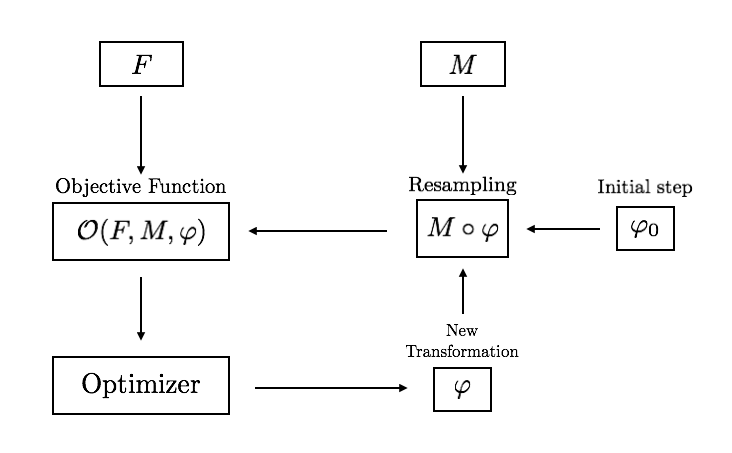
\includegraphics[scale=0.35]{figures/iterative_algorithm.png}
	\caption{Image registration framework scheme.}
	\label{fig:iterative_algorithm_scheme}
\end{figure}

\noindent
Modulating on the value of each knob, changing for example the set of transformation or the resampling technique, we change between the possible registration algorithms that generally falls in this framework.\\
%This is a simplification from which we can see that at each step, moving and fixed images are defined within their domain, not necessarily coincident. 

%Avoid the resampling at each iteration decreases computational time, reduces artifacts and enable to have more control on the consequence of the chosen resampling technique.
%
%\begin{figure}[!ht]
%	\centering
%	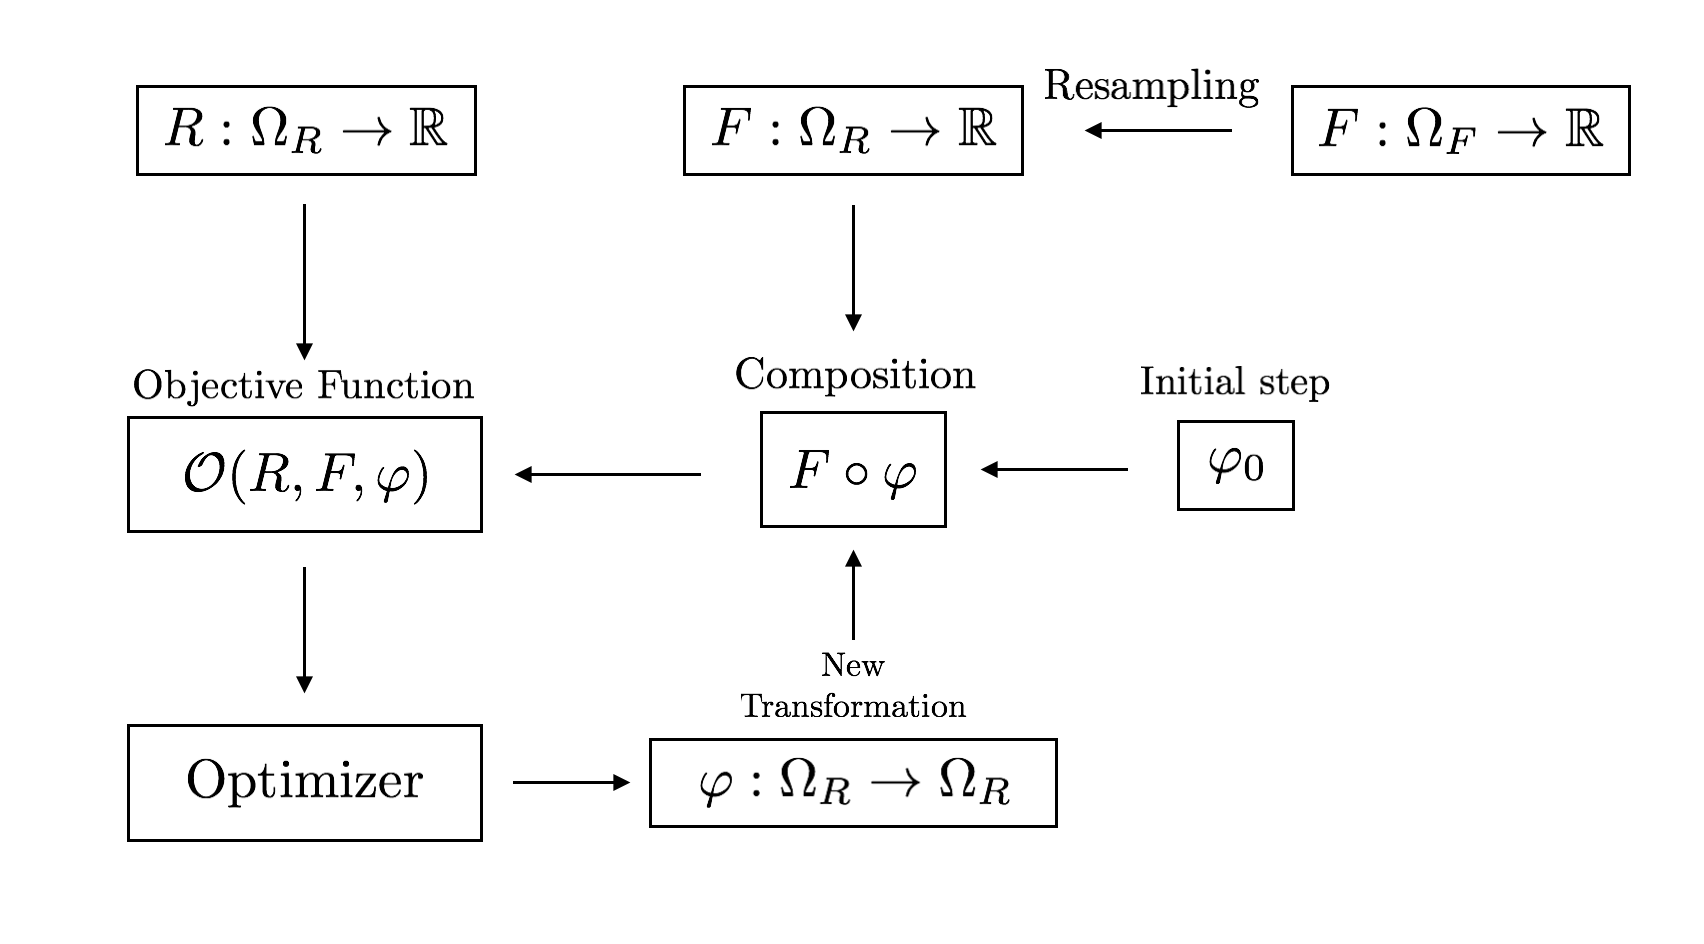
\includegraphics[scale=0.35]{figures/iterative_algorithm_res.png}
%	\caption{Image registration framework scheme.}
%	\label{fig:iterative_algorithm_scheme_modified}
%\end{figure}
\noindent
Far from being a complete overview of all of the possible frameworks, it does not take into account the fact that each version or implementation inevitably involves different needs and consequent challenges. Solutions found for each case may fall outside this simplification scheme: for example the parametrization of the transformations (or the deformation field's update) at each iterative step do not appear in this picture, even though is a fundamental feature. \\
In the following subsections we will going from the generalized framework to some specific algorithms. We are interestedin particular in the parametrization of the \emph{diffeomorphisms}\footnote{bijective differentiable maps with differentiable inverse; take the real valued $f(x)=x^3$: it is bijective differentiable but the inverse is not everywhere differentiable.} of the latest important algorithms: the LDDMM and the diffeomorphic Demons.

% % % % % % % % % % % % % % % % % % % % % % % % % % % % % % % % % % % % % %
% % SUB SECTION
% % % % % % % % % % % % % % % % % % % % % % % % % % % % % % % % % % % % % %
\subsection{LDDMM: Classic, Shooting and Stationary}

As previously done in the elastic registration \cite{Broit:1981}, the LDDMM framework \cite{beg2005computing} originates by considering motion between images as the motion of a fluid, and utilizes ODE from fluid dynamics to compute the deformation between reference and floating. 
Although, the discretized vector fields that can be stored in the computers' memory, are 5-dimensional matrix on a grid $G$ over the background space $\Omega$. The standard structure, used by most of the available software for image manipulation (\href{http://nipy.org/nibabel/}{Nibabel}, \href{http://niftilib.sourceforge.net/pynifti/intro.html}{py-NIfTI}, \href{http://niftilib.sourceforge.net/}{niftilib}, ...) is 
\begin{align*}
M = M(x_i,y_j,z_k,t,d) \qquad (i,j,k)\in G , ~~ t \in T  ~~ d = 1,2,3
\end{align*}
where $(x_i,y_j,z_k)$ are discrete position of the grid $G$, $t$ is the time parameter in a discretized domain $T$ and $d$ is index of the coordinate axis. So, the tangent vector $\mathbf{v}_{\tau}(x_i,y_j,z_k)$ at time $t$, has coordinates defined by
\begin{align*}
\mathbf{v}_{\tau}(x_i,y_j,z_k) = (M(x_i,y_j,z_k,t ,1), M(x_i,y_j,z_k,t,2), M(x_i,y_j,z_k,t ,3))
\end{align*}

Consider the set of homeomorphisms $\text{Hom}(\Omega)$ (continuous function from the background space $\Omega$ to itself with continuous inverse) that act\footnote{In this action it is preferable to consider the composition with the inverse, because this same action in differential geometry, called pull-back play the role of the contravariant operator of the push-forward, widely used to make a vector field act on a domain different from the one has been originally defined. For definitions on group's action and orbits, we refer to \cite{artin2011algebra}. For modern definitions of push-forward, pull-back and an introduction on Differential Geometry (in a non-Riemannian settings) \cite{lee2012introduction}.} on the set of images from the background space $\mathcal{I}_{\Omega}$:
\begin{align*}
\text{Hom}(\Omega) \times \mathcal{I}_{\Omega} & \longrightarrow  \mathcal{I}_{\Omega}   \\
(\varphi,F) &\longmapsto F\circ \varphi^{-1}
\end{align*}
its orbit, given an image $F$ and a subgroup of the homeomorphisms $\mathbb{G}\subset \text{Hom}(\Omega)$, consists in the set of the images having the same topology of $F$: 
\begin{align*}
\mathcal{E}_{\mathbb{G}}(F) = \{ F\circ \varphi^{-1} \mid \varphi \in \mathbb{G} \}
\end{align*}

The similarity term in the LDDMM is the $L^{2}$ norm\footnote{For an introduction on the $L^2$ norm in the continuous we refer to chapter 4 of \cite{stein2009real}.} between the moving image and the fixed image in the same orbit:
\begin{align*}
\text{Sim}(F,M,\varphi) = \frac{1}{\sigma^2}\euclideanMetric{F(\varphi^{-1})  - M  }_{L^{2}}^{2}
\end{align*}
while the regularization term that provides the optimal $\varphi$ at each step is defined on the norm of the velocity vector field tangent to the transformation. Limiting its length means impose a constrain on the speed of the transformation at each step. \\
Let $\text{Vect}(\Omega)$ be the set of all of the vector field over $\Omega$. A generic time varying vector field (TVVF) is the continuously differentiable map defined as
\begin{align*}
V:[0,1] & \longrightarrow  \text{Vect}(\Omega)\\
t  &\longmapsto  V^{(t)}  : \Omega \longrightarrow   \mathbb{R}^{d} \\
& \qquad \quad \quad ~~~\mathbf{x} \longmapsto V^{(t)}(\mathbf{x} )
\end{align*}
 Once initial conditions are given, at each TVVF, corresponds a unique time varying (or non-stationary) homomorphisms defined  by the following ODE 
\begin{align}\label{eq:ode_phi_v}
\frac{d\phi_{t} (\mathbf{x})}{dt} = V^{(t)}(\phi_{t}(\mathbf{x} ))
\end{align}
where 
\begin{align*}
\phi : [0,1] & \longrightarrow  \text{Hom}(\Omega)\\
t  &\longmapsto \phi_{t}  : \Omega \longrightarrow    \Omega \\
& \qquad \quad \quad  \mathbf{x} \longmapsto \phi_{t}  (\mathbf{x} )
\end{align*}
The transformation $\varphi$ between fixed and moving images ($ F\circ \varphi^{-1} = M $), can be defined by the couple $(V^{(t)},\phi_{t})$, such that, for $t = 0$, $\phi_{t} = Id$, identity of the group of homeomorphisms, and for $t = 1$, $\phi_{t} = \varphi$ is the sought homomorphism.
\begin{align*}
\varphi := \phi_{1} = \phi_{0} + \int_0^1 V^{(t)} (\phi) dt
\end{align*}
To have an efficient algorithm and a meaningful constraint on the resulting transformation, it is reasonable to consider $\phi_{t}$ as the shortest path between the identity and $\varphi$, so to have $V^{(t)} $ as the one that minimize the distance between transformations\footnote{This next equation can provide a metric on the manifold of the transformations, making it a Riemannian manifold. On the other side starting with a metric previously defined on the manifold (by a Levi-Civita connection so to be compatible with the shortest length of the integral curve), the consequent existence of geodesics may avoid the computation of the inf. In both cases this \lq\lq Riemannian approach\rq\rq  makes unavoidable the passage toward a metric, and makes the LDDMM a metric based algorithm.}:
\begin{align*}
l = \inf_{V^{(t)} ~ : ~ \dot{\phi_{t}} (\mathbf{x}) = V^{(t)}(\mathbf{x} )}  \int_{0}^{1} \euclideanMetric{V^{(t)}}_{L^2}^{2}dt
\end{align*}
Ending points of path on the set of diffeomorphisms, whose tangent vector field (that varies over time), are used as regularization term:
\begin{align*}
\text{Reg}(F,M,\varphi) =  \int_0^1  \euclideanMetric{L V^{(t)} }_{L^{2}}^{2}  dt
\qquad 
\dot{\phi_{t}} (\mathbf{x}) = V^{(t)}(\mathbf{x} ) 
\quad 
\phi_{0} = Id
\quad 
\phi_{1} = \varphi
\end{align*}
Were $L$ is a linear operator that can be dependent on some parameters that makes the approach even more general; it is defined as $L = (\alpha\vec \nabla^2 + \gamma)$ for $\alpha$ and $\gamma$ real parameters and $\vec \nabla^2$ the Laplace operator.
From the differential equation \ref{eq:ode_phi_v}, and in consequence of the definition of $\varphi$ the energy function \ref{eq:general_cost_function} become
\begin{align*}
%\argmin_{v_{t} ~ : ~ \dot{\phi_{t}} (\mathbf{x}) = v_{t}(\mathbf{x} ) } 
\mathcal{E}(F, M, \varphi) 
= 
%\argmin_{v_{t} ~ : ~ \dot{\phi_{t}} (\mathbf{x}) = v_{t}(\mathbf{x} ) } 
\int_0^1 \euclideanMetric{L V^{(t)} }_{L^{2}}^{2} dt + \frac{1}{\sigma^2}\euclideanMetric{F(\varphi^{-1})  - M  }_{L^{2}}^{2}
\end{align*}
And so the optimization algorithm, at each step of the registration will look for
\begin{align*}
\hat{V} 
= 
\argmin_{V^{(t)} ~ : ~ \dot{\phi_{t}} (\mathbf{x}) = V^{(t)}(\mathbf{x} ) } 
\int_0^1 \euclideanMetric{L V^{(t)} }_{L^{2}}^{2} dt + \frac{1}{\sigma^2}\euclideanMetric{F(\varphi^{-1})  - M  }_{L^{2}}^{2}
\end{align*}
Each transformation involved in the optimization algorithm are discretized time varying velocity fields; the update at each step is given by
\begin{align*}
\mathbf{v}_{k+1} = \mathbf{v}_{k} - \epsilon \nabla (\Delta\mathcal{E})
\end{align*}
where $\mathbf{v}^{k}$ is the $k$-th step of the approximation of the velocity vector field $V$, $\Delta\mathcal{E}$ is the discretized version of the energy function and $\epsilon$ is the gradient descent step size.\\

% shooting
A direct upgrade of the classical LDDMM performs the optimization on the geodesic flows, defined by a set of Hamiltonian equation (Shooting LDDMM \cite{vialard2012diffeomorphic}). \\
In this algorithm the iterative evolution of the deformation field, solution of the optimization algorithm, is regularized with the constraint imposed by an additional scalar field called \emph{initial momentum}. 
%stationary: dartel and hernandez
As proved by the authors, the evaluation of this constraint at each step provides geodesics flows of homeomorphisms, but it is computationally expensive. Using the log-euclidean framework presented in \cite{Arsigny:MRM:06}, the algorithm proposed in \cite{Ashburner:07} uses a constraint based on the stationarity of the involved velocity field. Instead of considering time varying velocity fields constrained by a set of Hamiltonian equations, the domain of vector field is reduced to the stationary, which is an -almost- equivalent constraint, that considerably reduces the computational complexity. Resulting algorithm, the DARTEL (Diffeomorphic Anatomical Registration using Exponentiated Lie Algebra), was published in contemporary with \cite{hernandez2007registration} based on the same concept of the parametrization of geodesics path of diffeomorphisms with stationary velocity fields, and with \cite{vercauteren2007non} that uses SVF on the Demons framework instead on the LDDMM.



% % % % % % % % % % % % % % % % % % % % % % % % % % % % % % % % % % % % % %
% % SUB SECTION
% % % % % % % % % % % % % % % % % % % % % % % % % % % % % % % % % % % % % %
\subsection{Demonology: Classic, Pasha, Diffeomorphic, Symmetric and LCC}

% classic demon
The first demons-based algorithm in image registration was proposed by \cite{thirion1998image} in analogy with the Maxwell's demon in thermodynamics. This early version, called classic (or additive) demons, do not involves diffeomorphisms; the floating image is deformed with a vector field resulting from the computation of the optical flow\footnote{Previously introduced for small deformation of optical sequence of images \cite{horn1981determining}.} regularized by a gaussian filter at each step. The optical flow is based on the idea that a voxel in the moving image is attracted by some force to all the points in the fixed with similar intensity, therefore it works under the hypothesis that the intensity of a moving object is constant over time. \\
Let $\mathbf{x}$ be a point in the background space $\Omega$, the unknown vector field $V:\Omega \rightarrow \mathbb{R}^{d}$ is the function that at each point satisfies:
\begin{align}\label{eq:optical_flow_initial}
V(\mathbf{x})\cdot \vec{\nabla}F(\mathbf{x}) = M(\mathbf{x}) - F(\mathbf{x})
\end{align}
Thus it can be defined pointwise as
\begin{align}\label{eq:optical_flow_pre}
V(\mathbf{x})
= 
\frac{(M(\mathbf{x}) - F(\mathbf{x}))\vec{\nabla}F(\mathbf{x})}{\euclideanMetric{\vec{\nabla}F(\mathbf{x})}^{2}  }
\qquad
\forall \mathbf{x} \in \Omega
\end{align}
To reduce the instability for small values of $\euclideanMetric{\vec{\nabla}F}$ and to satisfy the condition $V\rightarrow \mathbf{0}$ for little $\vec{\nabla}F$, the equation \ref{eq:optical_flow_pre} is multiplied by $\euclideanMetric{\vec{\nabla}F(\mathbf{x})}^{2}  / (\euclideanMetric{\vec{\nabla}F(\mathbf{x})}^{2} + (M(\mathbf{x}) - F(\mathbf{x}))^2)$:
\begin{align}\label{eq:optical_flow}
V(\mathbf{x})
= 
\frac{(M(\mathbf{x}) - F(\mathbf{x}))\vec{\nabla}F(\mathbf{x})}{\euclideanMetric{\vec{\nabla}F(\mathbf{x})}^{2}  + (M(\mathbf{x}) - F(\mathbf{x}))^2}
\qquad
\forall \mathbf{x} \in \Omega
\end{align}
Therefore, the classical demons algorithm defines the update of the transformation field at each step with \ref{eq:optical_flow} or with $V(\mathbf{x}) = \mathbf{0}$ when 
\begin{align*}
\euclideanMetric{\vec{\nabla}F(\mathbf{x})}^{2}  + (M(\mathbf{x}) - F(\mathbf{x}))^2 < \epsilon
\end{align*}
for $\epsilon$ spacing of floating point number.\\

%PASHA
In the paper that presents the PAHSA demons \cite{cachier2003iconic}, the authors underline the fact that the scalar product \ref{eq:optical_flow_initial} underpinning the classic demon consists in the minimization of a local energy function, one per volxel. They reformulate the algorithm using a global energy function, aimed to makes the method easier to be analyzed and compared with others. With some modification, the Classic demons algorithm is accompanied back to the framework presented in the previous section, having as energy function
\begin{align}
\mathcal{E}(F, M, C, V) = \frac{1}{\sigma_{s}}\text{Sim}(F,M,C) + \frac{1}{\sigma_{d}}\text{dist}(C,V) +  \frac{1}{\sigma_{r}}\text{Reg}(V) 
\end{align}
where $C$ and $V$ are both vector fields defined on the background space $\Omega$ and each $\sigma$ accounts for the uncertainty of each of the involved measure.\\
It differs from the energy function \ref{eq:general_cost_function} because of the additional \emph{hidden variable} $C$, whose purpose is to use alternating minimization algorithm\footnote{
	The optimization algorithm is divided in two phase: at the step $t$, in the first phase the first two addend of the energy function are optimized to obtain the approximation of $C$, $\mathbf{c}_{t}$ holding the variable $V$ to $\mathbf{v}_{t-1}$, approximation obtained from the previous step. In the second phase, the last two addend of the energy function are optimized to obtain the approximation of $V$ for $C$ keept constant at $\mathbf{c}_{t}$ obtained in the previous phase.
	} 
to optimize $\mathcal{E}$. Functions of involved in this new version of the energy function can be defined as
\begin{align*}
\text{Sim}(F,M,C) &= \euclideanMetric{ F - M\circ C  }^{2}\\
\text{dist}(C,V) &=\euclideanMetric{C - V}  \\
\text{Reg}(V)  &=\euclideanMetric{\vec \nabla V  }^{2}
\end{align*}
or with more advanced criteria proposed in \cite{cachier2003iconic}. In this context an equivalent version of the Classical demon, involving the global optimization function,can be reformulated from the preovious equations, keeping $C=V$:
\begin{align*}
\text{Sim}(F,M,V) &= \euclideanMetric{ F - M\circ V  }^{2}\\
\text{dist}(C,V) &=0 \\
\text{Reg}(V)  &=\euclideanMetric{\vec \nabla V  }^{2}
\end{align*}
and applying a Gaussian smoother at each step to regularize the solution.\\
The update of the vector field obtained with the optimization of the energy function and the Gaussian smoother is summed at each step with the previously computed vector field\footnote{This is the reason why in demonology, the classical demons is sometime classified as additive demon.}. Let $\{ \mathbf{v}_{j} \}$ be the vector fields' sequence approximating $V$ and $\delta\mathbf{v}$ the one computed at the iteration $j+1$ by the optimization algorithm, then the \emph{update} is computed with
\begin{align}\label{eq:additive_fields_composition}
\mathbf{v}_{j+1} := \mathbf{v}_{j} + \delta\mathbf{v}
\end{align}

% Diffeomorphic demons
Again the PASHA algorithm do not involves any diffeomorphism. This development was made in \cite{vercauteren2006robust}, with the diffeomorphic demons (or log-demon). 
Within the log-euclidean framework the involved vector fields are element in the tangent space of the group of diffeomorphisms. As in LDDMM, to each vector field $V \in \text{Vect}(\Omega)$ is associated a diffeomorphisms $p$ by the ODE $dp/dt = V^{(t)}(p) $.\\
In this settings, the update can not be computed simply with a sum, since it must reflect the composition of diffeomorphisms that defines the corresponding vector fields. Intuitively if $dp/dt = V^{(t)}(p) $ and $dq/dt = W^{(t)}(q) $ do not implies $dp\circ q/dt = V^{(t)}(p) + W^{(t)}(q) $.
To define the composition in the tangent space, we need to use two functions to transform vector fields into diffeomorphisms and vice-versa; they are already provided by Lie group theory. The \emph{Lie algebra}, usually denoted with $\mathfrak{g}$, contains the set of the tangent vector fields, while the Lie group, denoted with $\mathbb{G}$, contains the set of transformations; the function \emph{Lie exponential} maps vector fields on the corresponding Lie group elements while the \emph{Lie logarithm}, its inverse under some condition defined in chapter \ref{ch:tools}, maps each diffeomorphisms in the correspondent tangent vector field:
\begin{align*}
p = \exp(V)  
\quad
V = \log(p) 
\qquad \qquad
p \in \mathbb{G}
\quad
V \in \mathfrak{g}
\end{align*}
% update diffeomorphic demons
The addition of tangent vector fields \ref{eq:additive_fields_composition} that defines the update of the additive demons, becomes, in the diffeomorphic demon, the logarithm of the composition of the two diffeomorphisms that corresponds to the vector fields in the Lie group:
\begin{align}\label{eq:first_log_composition}
\mathbf{v}_{j+1}= \log(\exp(\mathbf{v}_{j})\circ\exp( \delta\mathbf{v}))
\end{align}
And again the theory of Lie group provides a formula to compute this composition: the BCH formula. This involves an infinite series of nested Lie bracket, that do not makes its computation a straightforward task: 
\begin{align*}
BCH(\mathbf{v}_{j},\delta\mathbf{v}) 
:= 
\mathbf{v}_{j} + \delta\mathbf{v} + \frac{1}{2}[\mathbf{v}_{j},\delta\mathbf{v}] + \frac{1}{12}([\mathbf{v}_{j},[\mathbf{v}_{j},\delta\mathbf{v}]]
+ [\delta\mathbf{v},[\delta\mathbf{v},\mathbf{v}_{j}]])  +... 
\end{align*}
Remarkably, if we set to $0$ all the lie brackets in the BCH formula (so we neglect the curvature of the space), the resulting composition of vector field in the log domain will coincide with \ref{eq:additive_fields_composition}: 
\begin{align*}
BCH(\mathbf{v}_{j},\delta\mathbf{v}) 
\simeq 
\mathbf{v}_{j} + \delta\mathbf{v} 
\end{align*}

% IMAGE additive demons - diffeomorphic demons
	\begin{figure}[!ht]
		\centering
		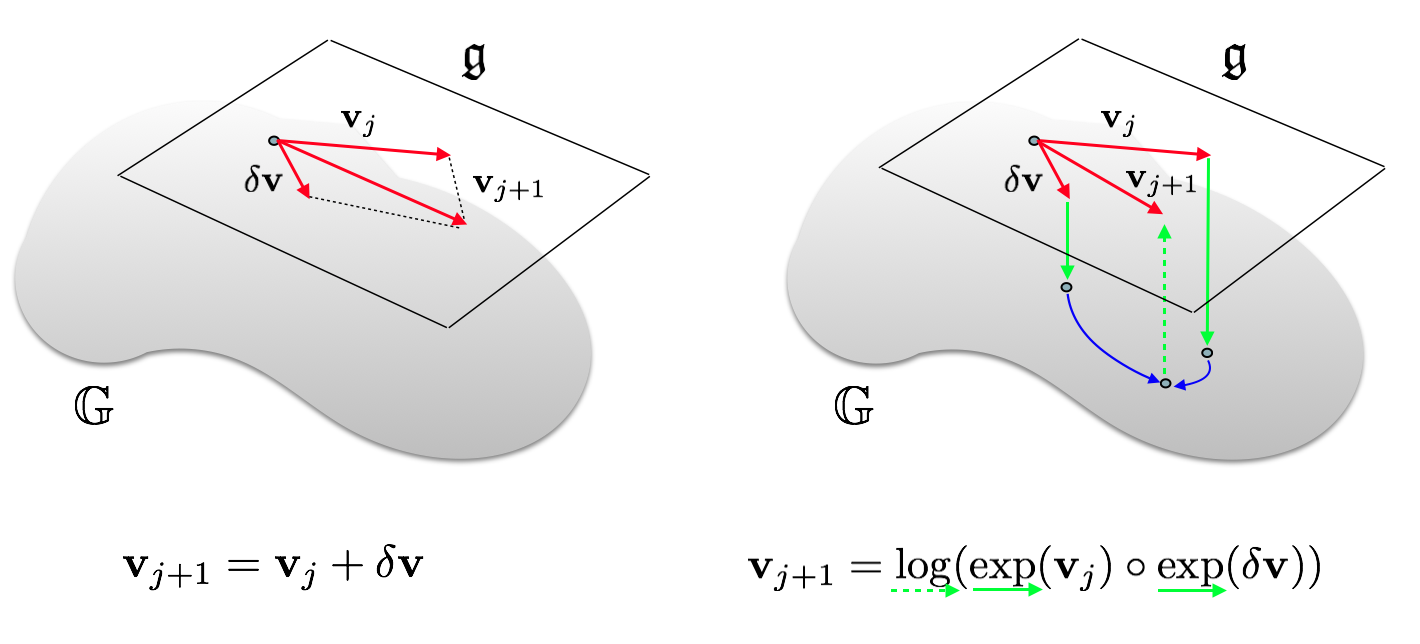
\includegraphics[scale=0.27]{figures/add_diff_demons.png}
		\caption{Each update computed in the additive demons algorithm is the sum of vector fields (left). In diffeomorphic demons algorithm vector fields are considered as elements of the lie algebra $\mathfrak{g}$, tangent space of the Lie group of diffeomorphisms. The update is compute as the composition of the correspondent transformations in the Lie group $\mathbb{G}$ using the canonical transformations $\exp$ and $\log$ (right).}
		\label{fig:additive_diffeomorphic_demons}
	\end{figure}  
%  Symmetric diffeomorphic demon
An extension of the diffeomorphic demons, that involves the optimization of the energy function $\mathcal{E}(F,M,V) $, exploits the existence of the inverse transformation and optimizes instead a symmetrised version of the energy function \cite{vercauteren2007non}. If $V = log(p)$, then the \emph{symmetric diffeomoprhic demons algorithm} finds at each step
\begin{align*}
\tilde{V}_{t+1} 
= 
\argmin_{p \in \mathbb{G} } 
\mathcal{E}(F,M,log(p)) + \mathcal{E}(F,M,\log(p^{-1})) 
\end{align*}

% LCC diffeomorphic demon
A further development of the diffeomoprhic demons algorithm, presented in \cite{lorenzi2013lcc}, preserve the structure of the symmetric version, but uses the LCC measure of similarity instead of $L^{2}$ to compute the energy function.\\

Last section of this chapter is devoted to introduce the intuition of this concept, while chapter \ref{ch:tools} is devoted to the introduction the formal definitions and to its development.


% % % % % % % % % % % % % % % % % % % % % % % % % % % % % % % % % % % % % %
% % SECTION
% % % % % % % % % % % % % % % % % % % % % % % % % % % % % % % % % % % % % %
\section{The Composition of SVF in the Diffeomorphisms Group}

Every non-rigid registration algorithm requires to be implemented and to work with discretized images.
The nature of the computers' memory prevent from the possibility of storing the continuous fluid transformations that solves the differential equations of the LDDMM and the diffeomorphic demons approach: the only thing that we can do, unfortunately, is to store the discretized vector fields and resampling them with the images using one of the available techniques.\\
% why log composition:
When relying on diffeomorphisms, we still have to consider discretized vector fields as input and output, but we need the Lie group of diffeomorphisms as support to compute the composition \ref{eq:first_log_composition} from the tangent space.
This operation is baptized under the name of \emph{log-composition} and it is defined as
\begin{align*}
U \oplus V := \log(\exp(U)\circ\exp( V))
\qquad \qquad
\forall U, V \in \mathfrak{g}
\end{align*}
The main aim of this research is to find and compare numerical ways to compute it. \\

% where we can use the log composition
A fast log-composition is not useful only for the diffeomorphic demons. It can be used to solve every problem that uses Lie groups and need to be implemented in a computer. In medical imaging it can be used for
\begin{enumerate}
	\item Diffeomorphic demon, and symmetric diffeomorphic demon \cite{vercauteren2006robust, vercauteren08}.
	\item Fast computation of the logarithm \cite{Bossa:08}.
	\item Calculus on diffusion tensor \cite{Arsigny:MRM:06}. 
	\item Compute the discrete ladder for Parallel Transport in Transformation Groups \cite{Lorenzi:discrete_ladders:14}.
\end{enumerate}	
	
The next chapter is devoted to the formal definition of the log-composition, underpinned with the tools from differential geometry theory and to present the numerical technique developed so far to compute it.







%Under this light, the transitions from the Lie group to Lie algebra (the Lie logarithm) and its return (the Lie exponential) become fundamental tools.
%The main topic of this research is the evaluation of the operation that we define here as \emph{Lie algebra Group Composition}, or simply \emph{Group Composition}, 
%
%
%
%
%One of the Matrix Lie group explored in this research is the special euclidean group $\text{SE}(d)$, or group of rigid transformations.
%A little increase in the number of degrees of freedom leads to the group of the affine transformations, where scaling and shearing have been added to the possible transformations. \\
%The idea of maximize the number of degrees of freedom in a transformation that maintains anatomical features between images, led to consider the Lie group of diffeomorphism $\text{Diff}$.
%A diffeomorphism $p$ can be expressed as the sum of the identity function with a differentiable transformation depending on $\mathbf{x}$. It is possible to write:
%\begin{align*}
%p(\mathbf{x})  = \mathbf{x} + \gamma(\mathbf{x})
%\end{align*}
%With this notation the vector $\dot{\gamma}(\mathbf{x})$ is the speed\footnote{as we will see, a feasible way to express a set of diffeomorphisms is as the solution of the differential equation defined by the velocities of the transformation.} of each point from its original to a new position due to the application of $p$.\\
%In the iterative diffeomorphic registration algorithm (in which the structure is defined by regularization and similarity), to obtain the update at each step, it is required to apply consecutively two diffeomorphisms $p_{i}$ and  $\hat{p}_{i+1}$ and consider the resulting composition as the required update.
%%\begin{figure}[!ht]
%%	\centering
%%	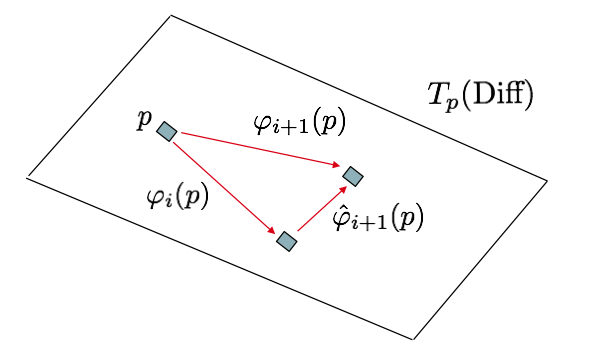
\includegraphics[scale=0.35]{figures/diff_update.png}
%%	\caption{Composition of tangent vectors of diffeomorphism (provisional).}
%%	\label{fig:composition1}
%%\end{figure}
%As a consequence, the corresponding vector of the transformation $p_{i+1}$ in the tangent space of the Lie group can be computed, given two vectors in the tangent bundle, with an operation called here \emph{the group composition in the Lie algebra}.\\
%In \cite{Bossa2007} the BCH formula appears as an improvement of the scaling and squaring algorithm to compute the logarithm of a matrix. As noticed in the same paper, the BCH formula is used in a infinite dimensional settings, while its validity has been proven only for finite dimensional Lie group. In addition while composing the logarithm of a composition of two exponentials, the initial tangent vectors belongs to the same tangent space. This is not the case while composing $p_{i}$ with $\hat{p}_{i+1}$ the tangent vector that defines $\hat{p}_{i+1}$ is an element of the tangent plane to $p_{i}$. \\
%Is it possible to reach a proper computation thanks to the definition of Affine exponential, that differs from the Lie exponential used in \cite{Bossa2007} .
%
%
%
%
%
%
%The BCH formula provides an expression of the Group Composition in the finite dimensional case expressed as an infinite series of nesting commutators. The difficulties involved in dealing with this formula, as well as its non completely proper use in the infinite dimensional setting, gave birth to some methodologies and approaches, whose investigation is the main goal of this research. One of these approaches, involves the Taylor expansion and has a computable form in the finite dimensional. A geometrical approach that holds also in the infinite dimensional case is the parallel transport.
%It can be considered as a natural approach to evaluate the group composition with offset. It consists in the transport of the vector $\mathbf{v}$ along the geodesic having $\mathbf{u}$ as tangent vector such that during the transport it maintains the condition of parallelism. The resulting vector $\mathbf{v}^{\parallel}$ in the tangent plane of $\mathbf{u}$ can be then summed with $\mathbf{v}$ with similar results to the direct application of the BCH. Its evaluation involves the Schild's ladder and the pole ladder. Both have already found practical application in medical imaging \cite{Lorenzi:discrete_ladders:14}, \cite{Lorenzi:pt:13}.
%Parallel transport is necessarily related with the definition of the connection. Choosing among possible connections become a crucial feature, whose consequences in the corresponding realization in the transformation of images requires further studies.
%
%\begin{figure}[!ht]
%	\centering
%	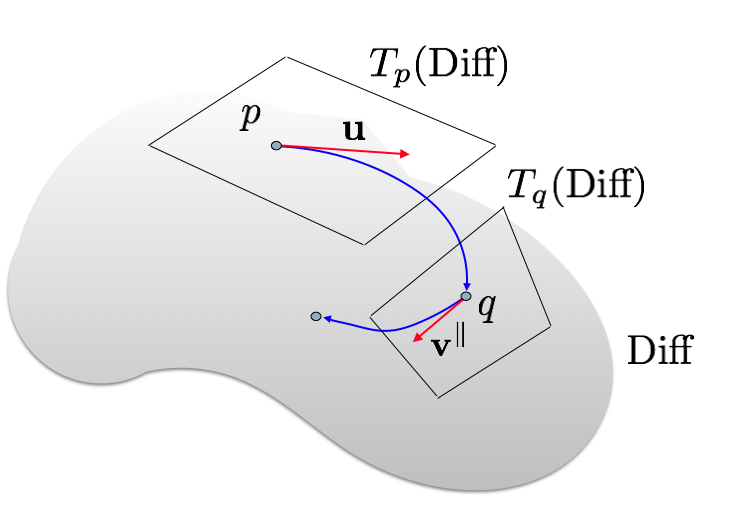
\includegraphics[scale=0.25]{figures/parallel_transport_1.png}
%	\caption{Group composition with offset using parallel transport.}
%	\label{fig:composition}
%\end{figure}
%
%The lack of a close form of any kind and the theoretical difficulties inherent to the investigation of infinite dimensional group of diffeomorphism makes an experimental approach meaningful. 





